\documentclass[11pt, a4paper,twoside]{report}

\usepackage[utf8]{inputenc}
\usepackage[english]{babel}
\usepackage{amsmath}
\usepackage[T1]{fontenc}
\usepackage{amssymb}
\usepackage{indentfirst}
\usepackage{subfigure}
\usepackage[version=4]{mhchem}
\usepackage[font=small,labelfont=bf]{caption}

\usepackage[nottoc]{tocbibind}

\usepackage{geometry}
 \geometry{a4paper,
 left=3cm,
 top=3cm,
 bottom=3cm,
 right=2.5cm
 }

\usepackage{graphicx}
\graphicspath{ {./figures/} }


% Fancy Headers

\usepackage{fancyhdr}
\pagestyle{fancy}
%\renewcommand{\chaptermark}[1]{%
%\markboth{\MakeUppercase{\small #1}}{}}
\renewcommand{\headrulewidth}{0pt}

\fancyhead[LE]{\slshape\nouppercase \rightmark} %section
\fancyhead[RE]{\thepage}
\fancyhead[RO]{\slshape\nouppercase \leftmark} % chapter
\fancyhead[LO]{\thepage}

\usepackage{algorithm} 
\usepackage{algpseudocode} 


%\usepackage{palatino}

\newcommand{\twopartdef}[4]
{
	\left\{
		\begin{array}{ll}
			#1 & \mbox{if } #2 \\
			#3 & \mbox{if } #4
		\end{array}
	\right.
}


\begin{document}
	\pagenumbering{roman}
	
	\addcontentsline{toc}{chapter}{Contents}
	\tableofcontents
	\listoffigures
	\listoftables
	
	\newpage
	
	\pagenumbering{arabic}

	\chapter{Ferromagnetism and the Ising Model}

\section{Ferromagnetism}

\begin{figure}[h]
	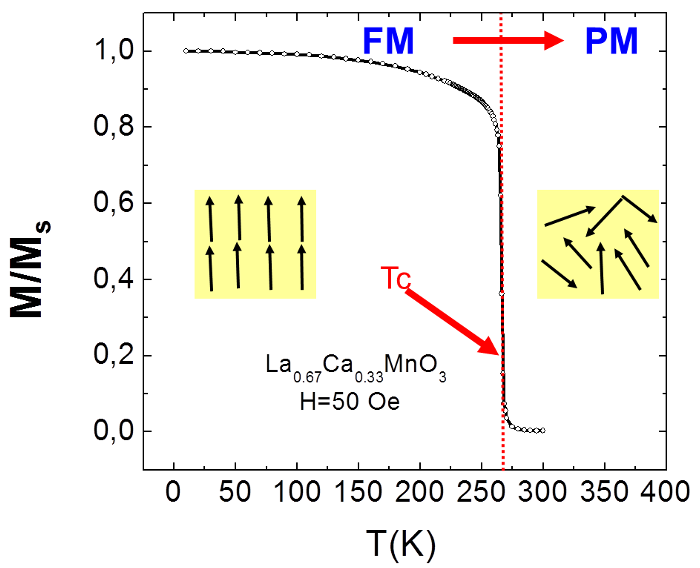
\includegraphics[scale=1]{phase_transition.png}
	\centering
\end{figure}

\begin{figure}[h]
	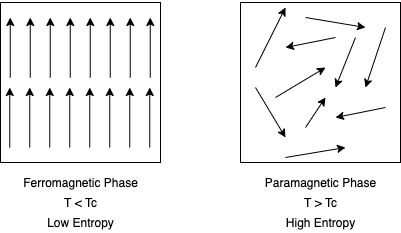
\includegraphics[scale=0.5]{spins_diagram.png}
	\centering
\end{figure}


\section{Ising Model}

\subsection{Joint Density of States}


\begin{figure}[h]
	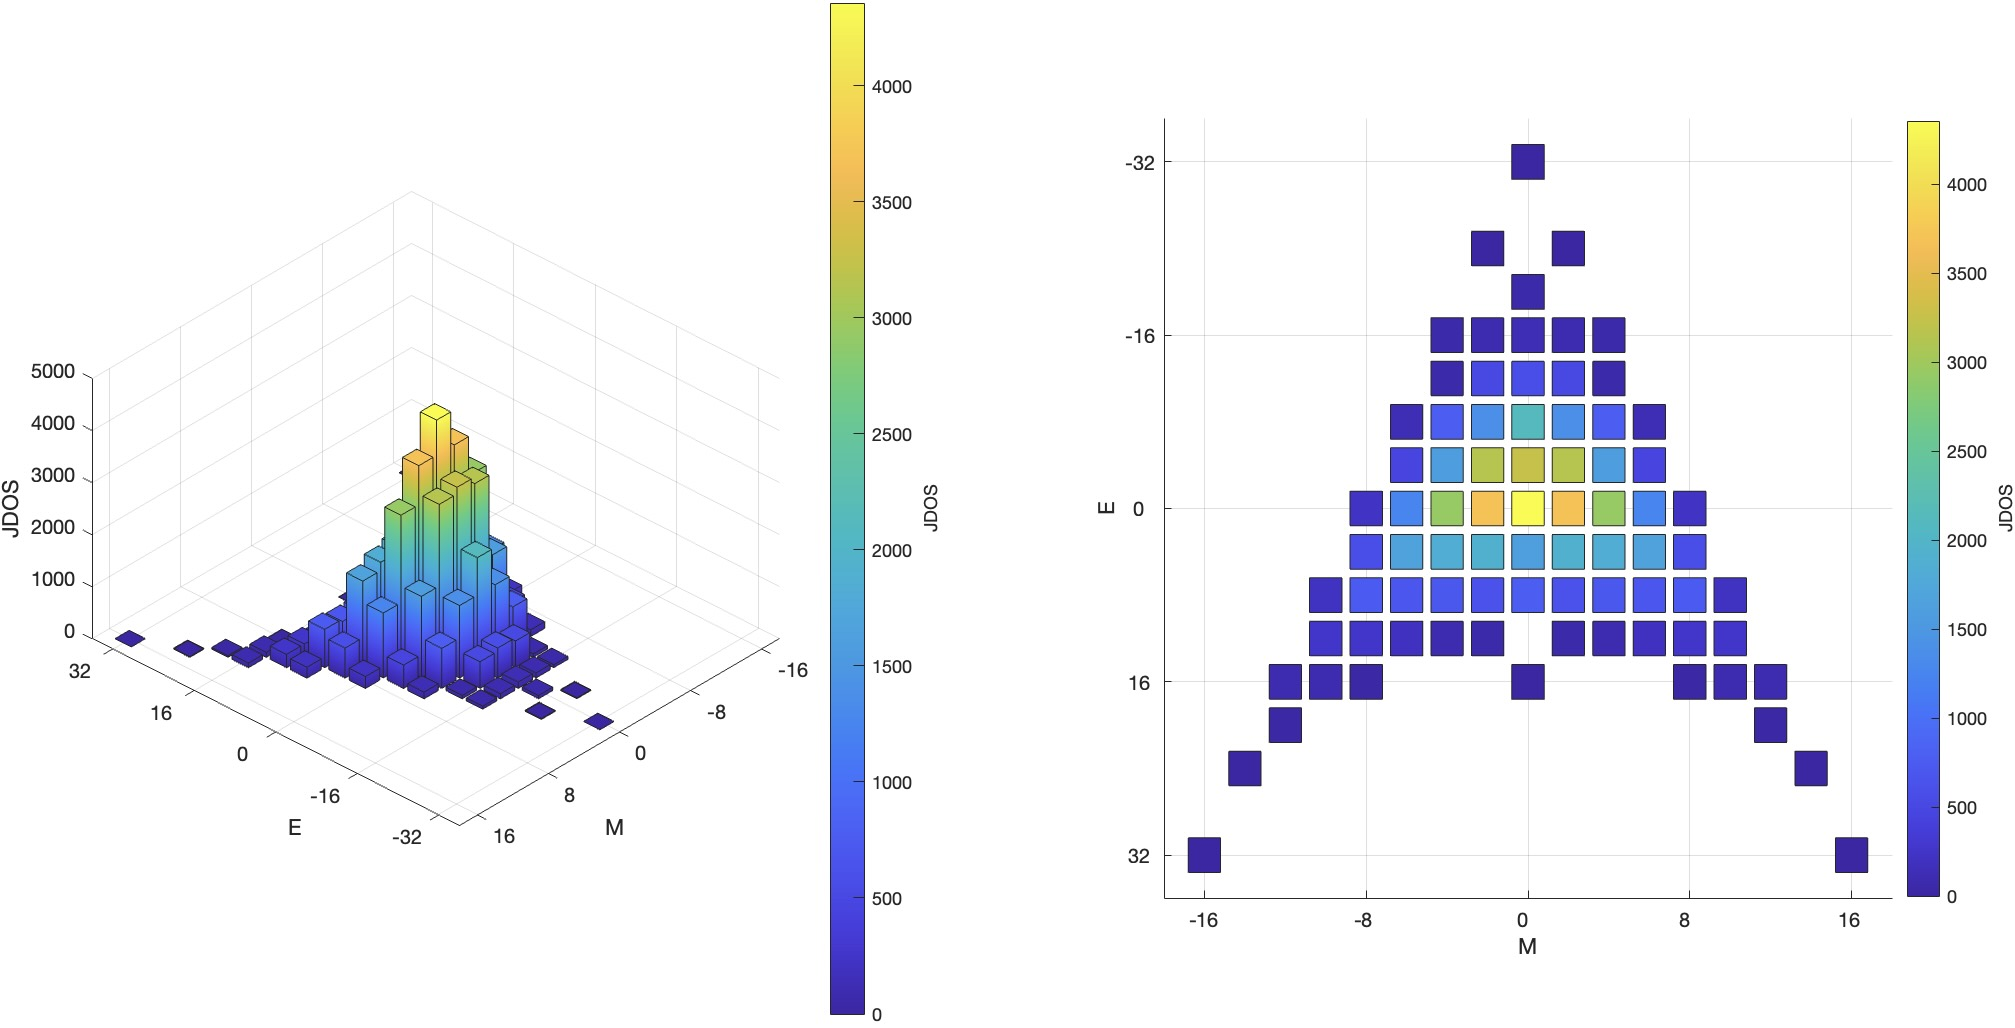
\includegraphics[scale=0.2]{JDOS_exact_L4_SS.jpeg}
	\centering
\end{figure}





\subsection{Thermodynamics}

\subsection{Relevance}
	\chapter{Monte Carlo Methods Applied to the Ising Model}

A short review of the Monte Carlo (MC) methods used to solve the Ising Model in the current paradigm is presented. There will be a focus on the famous Metropolis Method and the Wang-Landau sampling. 

\section{Metropolis Method}

The classic Metropolis method, introduced in 1953 by Metropolis et al., belongs to the Markov chain Monte Carlo (MCMC) class of algorithms. These algorithms exploit the fact that if we construct a Markov chain that has a specific equilibrium distribution one can obtain samples recording the states generated by the Markov chain. 

In a brief fashion, a Markov chain is a stochastic model that describes a sequence of possible events, in this case microstates,in which the probability of transiting to another state depends on the current state. This way the probability of the next state, $S_j$, given the current state, $S_i$, can be written as 
\begin{equation}
	P(S_j, t) = \sum_i W(S_i \rightarrow S_j) P(S_i, t),
\end{equation}
where $W(S_i \rightarrow S_j) \equiv W_{ij}$ is the transition probability to move from the state $i$ to $j$. We require that 
\begin{equation}
	W_{ij}  \geq 0 \quad \quad \quad \quad \quad \sum_j W_{ij}=1.
\end{equation}
The master equation considers the change of the probability of the next state with time, $t$,
\begin{equation}
	\frac{dP(S_j, t)}{dt} = \sum_i \left[ W_{ij}P(S_i, t) - W_{ji} P(S_j,t)  \right].
\end{equation}
In the equilibrium regime, the master equation has to equal $0$, and we get the detailed balance condition for the equilibrium probability $P_{eq}(S_j)$,
\begin{equation}
	W_{ji}P_{eq}(S_j) = W_{ij}P_{eq}(S_i).
\end{equation}

The object of Metropolis Sampling is to generate canonical configurations with an equilibrium probability
\begin{equation} \label{eq:met_prob_eq}
	P_{eq}(E_i) = \frac{\exp(-\beta E_i)}{Z}.
\end{equation}
Here $Z$ is the partition function, however this is usually not know before hand. When considering a Markovian process we generate each new configuration from the preceding one avoiding this problem. As a result the difference of energy between the two states is needed, $\Delta E = E_i - E_j$ and the transition probability of given as

\begin{equation}
	W_{ij} = \twopartdef { \tau_0^{-1} \exp(-\beta \Delta E) } {\Delta E \geq 0} {\tau_0^{-1}} {\Delta E < 0}
\end{equation}
where $\tau_0^{-1}$ is the time required to attempt a spin-flip.  We often set this time unit to one.

This way the Metropolis method applied to the Ising Model, with a fixed external magnetic field and a fixed temperature, goes as follows:

\begin{enumerate}
\item Choose an initial state;
\item Choose a spin $i$ and perform a spin-flip;                                                                                                                                       
\item Calculate the energy change from that spin-flip, $\Delta E$;
\item Accept the flip with a probability $\min \left( 1, \exp(-\beta \Delta E) \right)$; 
\item When the system reaches equilibrium, measure any thermodynamic quantity needed;                                                                                                        
\item Go back to (2) and repeat until there is enough samples of the thermodynamic variables.                                                                                                                    
\end{enumerate}
Note that we accept the spin flip if a given uniformly random number $r, r \in [0,1]$, is less or equal to the acceptance criteria. Typically in Monte Carlo simulations we define the MC time as the amount of trial flips equal to the number of spins in our lattice, N.

\subsection{Success and Limitations}

The Metropolis sampling proposed by Metropolis et al., can be successfully applied to an array of models, ranging from widely studied quantum ensembles and gases simulations to state-of-the-art protein and peptide simulations and to machine learning and neural networks. The following paragraphs will be directed to magnetic systems, like the Ising model, but they can be extrapolated to others physical systems. 

When getting thermodynamic variables we have to let the simulation reach the equilibrium stage, where the probability distribution takes the form of equation \ref{eq:met_prob_eq}. Then we take a measurement each MC time, resulting in $M$ total values for that variable. At the end the average if that variable, $A$, is taken $\langle A \rangle = \frac{1}{M} \sum_i A_i$. 
For large systems the time taken to reach equilibrium stage is often very long thus making the simulation time consuming. 
This is worsened by the fact that to study how some thermodynamic variable $A$ changes over a wide range of temperatures or applied fields intensities, we need to run multiple Metropolis simulations for each temperature and field intensity values, making this process very time-consuming.

Lastly there is another shortcoming known as critical slowing down. In short, for computations where the temperature is near the critical temperature, $T_C$, the sampling slows down, meaning that it is more time-consuming for the computations to reach the equilibrium stage, thus slowing down the overall simulation.

\section{Wang-Landau Sampling}

Since its introduction, the Metropolis sampling was the go-to method to study phase transitions and critical phenomena in condensed matter physics and statistical mechanics. In the final decades of the 20th century scientists were committed to develop new methods that could overcome the shortcomings of the Metropolis Sampling. Various methods were proposed such as the cluster flip algorithms, where Swendsen and Wang where pioneers, and the multicanonical ensemble method. The first solved the critical slowing down present in the Metropolis and the second could sample rough energy landscapes with ease. 

In 2001, Fugao Wang and David P. Landau proposed a new Monte Carlo method, now called the Wang-Landau (WL) method or sampling. The goal of this method diverges from the goal of previous methods. Instead of generating configurations with a canonical probability, this method tries to estimate the canonical partition function
\begin{equation}
	Z = \sum_E g(E) \exp(-\beta E)
\end{equation}
through the estimation of the density of states $g(E)$ from a flat histogram in the phase space.

The main difficulty of a simple random walk in the energy space is that the walker would spend most of its time in the highest probable states thus making the random walk ineffective. The idea of the Wang-Landau sampling is to do a random walk,Metropolis like, and accepting the new states with a probability proportional to the inverse to their DoS $\frac{1}{g(E)}$. Doing this we obtain a flat histogram meaning that each macrostate has the same probability of being visited.  
Since $g(E)$ is unknown \textit{à priori}, in each step of the random walk, $g(E)$ is also being constructed.

The proposed algorithm computed the DoS but, it can also estimate the JDoS by performing the random walk in the phase space composed by energy, $E$, and the second order parameter, in our case, the magnetization of the system, $M$. This comes with a downside, since the JDoS has 1000x more information than the DoS it takes 1000x more time to compute.
Later in 2006, Landau, presented a modification of the WL called the global updates method. This is a much harder version to implement but is much more efficient when sampling 2D discrete phase spaces and continuous phase spaces. 

\subsection{Algorithm}

First we start with an arbitrary configuration of spins and a guess for the density of states. Usually,this  guess is $g(E, M)=1$. Choosing a random site in our lattice, we perform a trial flip and compute the energy-magnetization pair before the trial, $(E_i, M_i)$, and after, $(E_j,M_j)$. The new configuration is accepted with a probability
\begin{equation}
	P((E_i, M_i) \rightarrow (E_j, M_j)) = \min\left(1, \frac{g(E_i, M_i)}{g(E_j, M_j)}\right).
\end{equation}
Whether the configuration is accepted or rejected, we have to update the histogram and refine the DoS estimation. This way, being the system in the state $(E, M)$,
\begin{equation*}
	H(E, M) = H(E,M)+1,
\end{equation*}
and we multiply the current value of the DoS by a modification factor, $f > 1$,
\begin{equation*}
	g(E,M)=fg(E,M).
\end{equation*}
A reasonable choice for the initial value of the modification factor if $f_0 = e$. If $f_0$ is too small, the simulation will take a very long time to reach all of the possible macrostates, $(E,M)$. If it is too large, then we will have large statistical errors.  
This process is repeated until the histogram is considered "flat", all of the possible energies have been visited the same number of times. As it is impossible to obtain a $100\%$ flat histogram, we define a rule for flatness as $\min(H(E, M)) > \langle H(E, M) \rangle \times p$; $p$ is chosen according to the size of the problem. For small cases, such as the two dimensional Ising model, $p$ can be set as high as $0.95$, but for larger systems the flatness condition may never be satisfied if $p$ is near unity.  
Once a flat histogram is reached, we set $H(E, M)=0$, keep the estimation of the DoS and reduce the modification factor, $\sqrt{f_{i}} \rightarrow f_{i+1}$ and continue the random walk. We stop the simulation if $f<f_{final}$, where $f_{final}$ is a number very close to one (often $f_{final} \sim 1+1E-8$). 

At the end, the method gives us the relative density of states. To determine the normalized DoS we can use the fact that 
\begin{equation}
	\sum_{E,M} g(E,M) = 2^N.
\end{equation}

\subsection{Success and Limitations}

The modification factor controls the accuracy and the steps taken to reach a flat histogram in our computations. As it approaches unity, the number of iterations goes to infinity. This way, at the beginning of the simulation, when the modification factor is large, the estimation of the DoS is quite bad, since there we are taking fewer samples with a high weight. At the later stages, the modification factor is lower therefore we have more samples of each macrostate with a lower overall weight. 
Therefore, the initial stages of the simulation are characterized by the accumulation of low precision statistics and the later stages by the refining of the firsts samples. 

\begin{figure}[h]
	\centering
	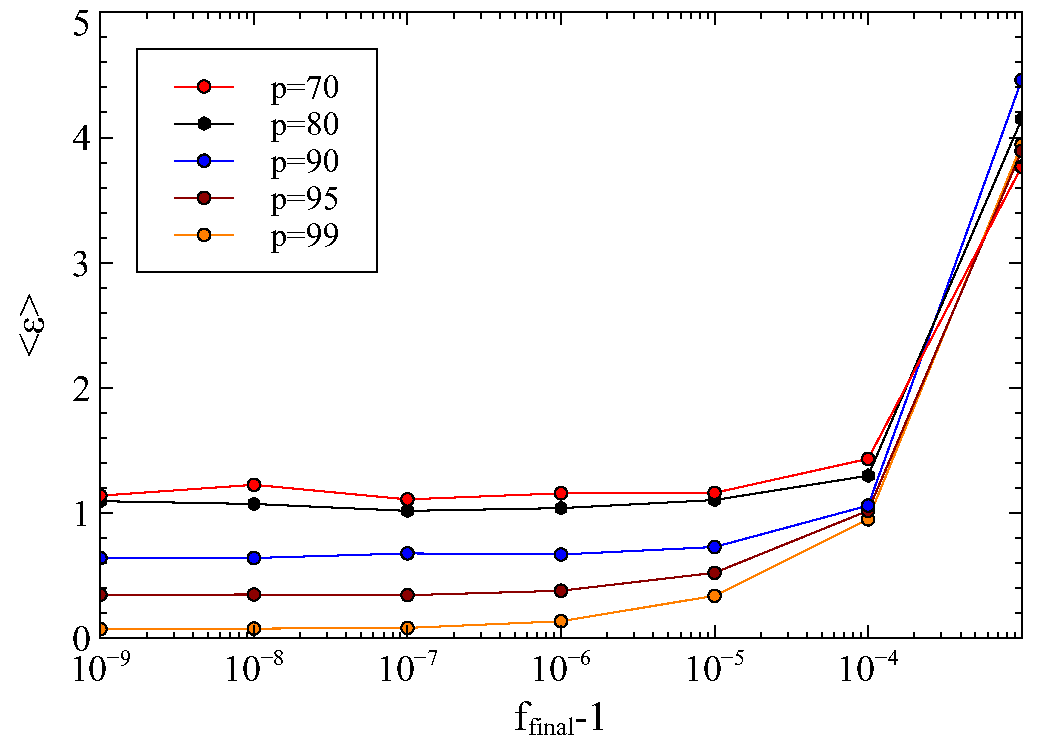
\includegraphics[scale=0.6, height=6cm]{wl_mean_error_f.pdf}
	\caption{TODO: MORE P VALUES!!!! REMOVE ERROR BARS! Mean absolute error of the JDoS for the Ising model computed by the Wang-Landau sampling for a L4 SS lattice plotted against $f_{final}-1$. The flatness condition used was 90\%.}
	\label{error_abs_wl}
\end{figure}

Due to the wrong samples at the initial stages of the computations, the final estimation of the JDoS will converge to the exact solution, but the mean error in our computations will never vanish, independent of the flatness criteria used, shown in figure \ref{error_abs_wl}. 

A few modifications to the original WL were proposed throughout the years, but the most noteworthy  are the modifications from Belardinelli et al. and from Chenggang Zhou et al.. The former has studied the method in great detail and was a co-author of the global updates method. He proposed the introduction of a parameter $S$, defined as the separation between successive records in the histogram. Meaning that in our random walk we would only update the histogram each $S$ steps. This will diminish the correlation between successive samples and improve accuracy.  

\begin{figure}[h]
	\centering
	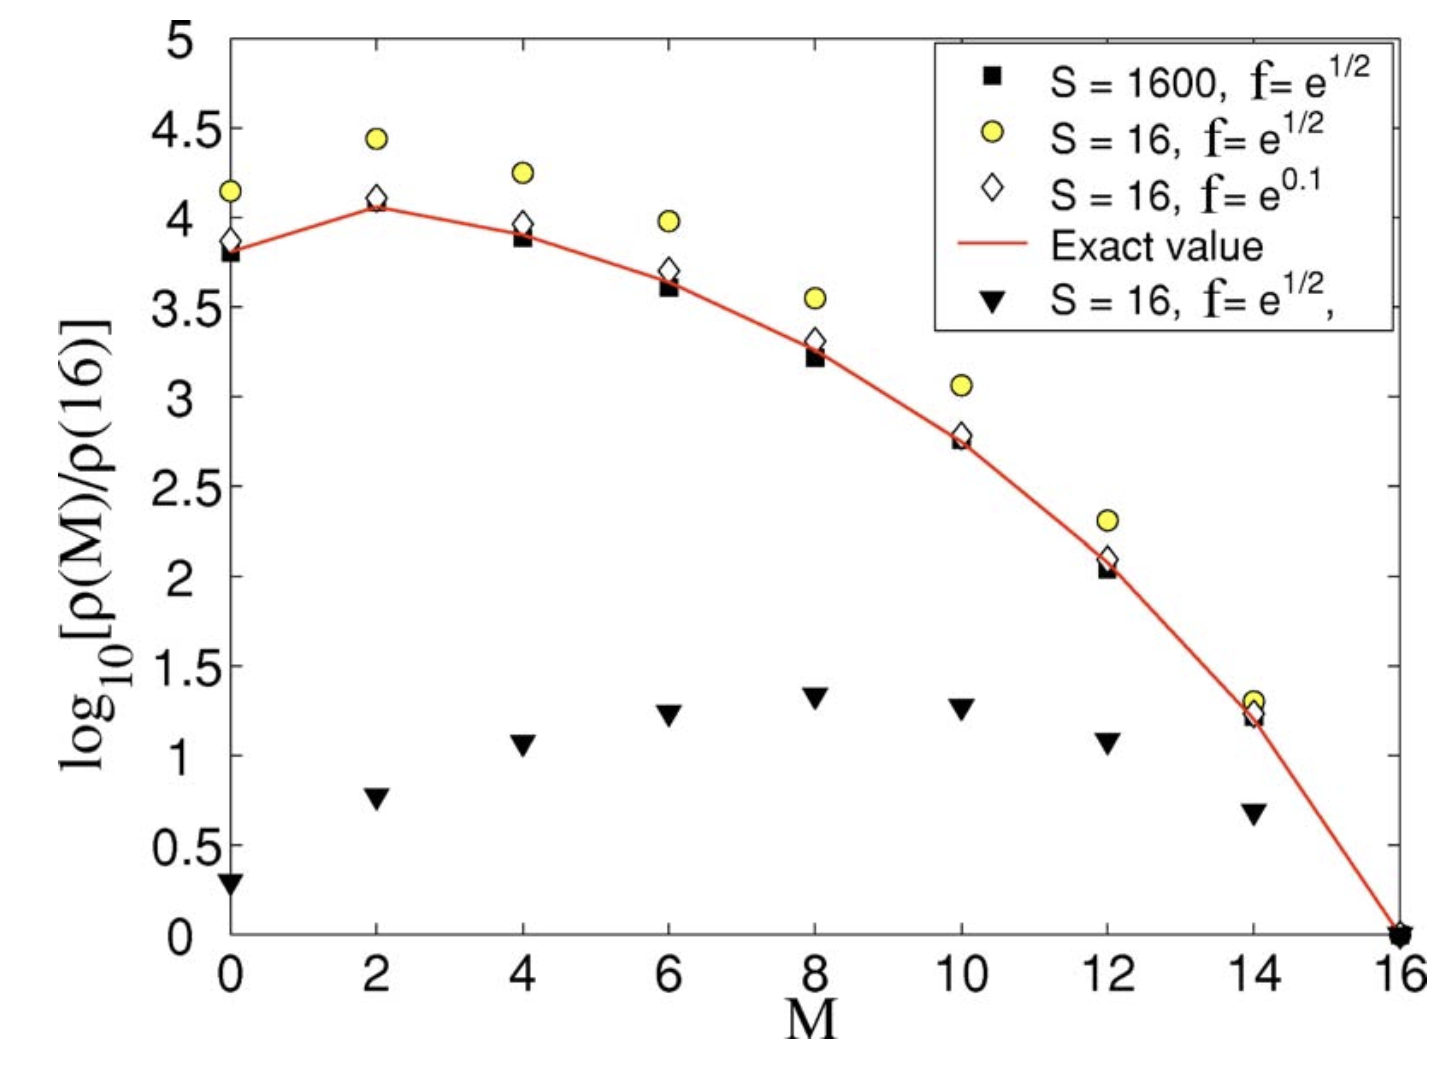
\includegraphics[scale=0.6, height=5.5cm]{S_paper_fig.png}
	\caption{$g(M)$, the density of states for magnetization $M$ of L4 SS Ising lattice normalized. The solid line connects the exact values, and the symbols were obtained with different parameters $f$ and $S$. Data was averaged over $100$ measurements, so the statistical errors are smaller than the symbols. Taken from .}
	\label{S_parameter}
\end{figure}

The modification proposed by Belardinelli et al. is more complex and introduces a new way of changing the modification parameter during the computations, they called it the $1/t$ time-dependent algorithm. The method starts as the WL does, however, if $f_{i+1} \leqslant 1/t$, where $t$ is the MC time, the modification factor becomes $f_{i+1} = f(t) = 1/t$ and we discard the histogram and update $f$ each MC time step. The simulation only stops when $f(t) < f_{final}$. This ensures that the mean error vanishes, figure \ref{t_algorithm}.

\begin{figure}[h]
	\centering
	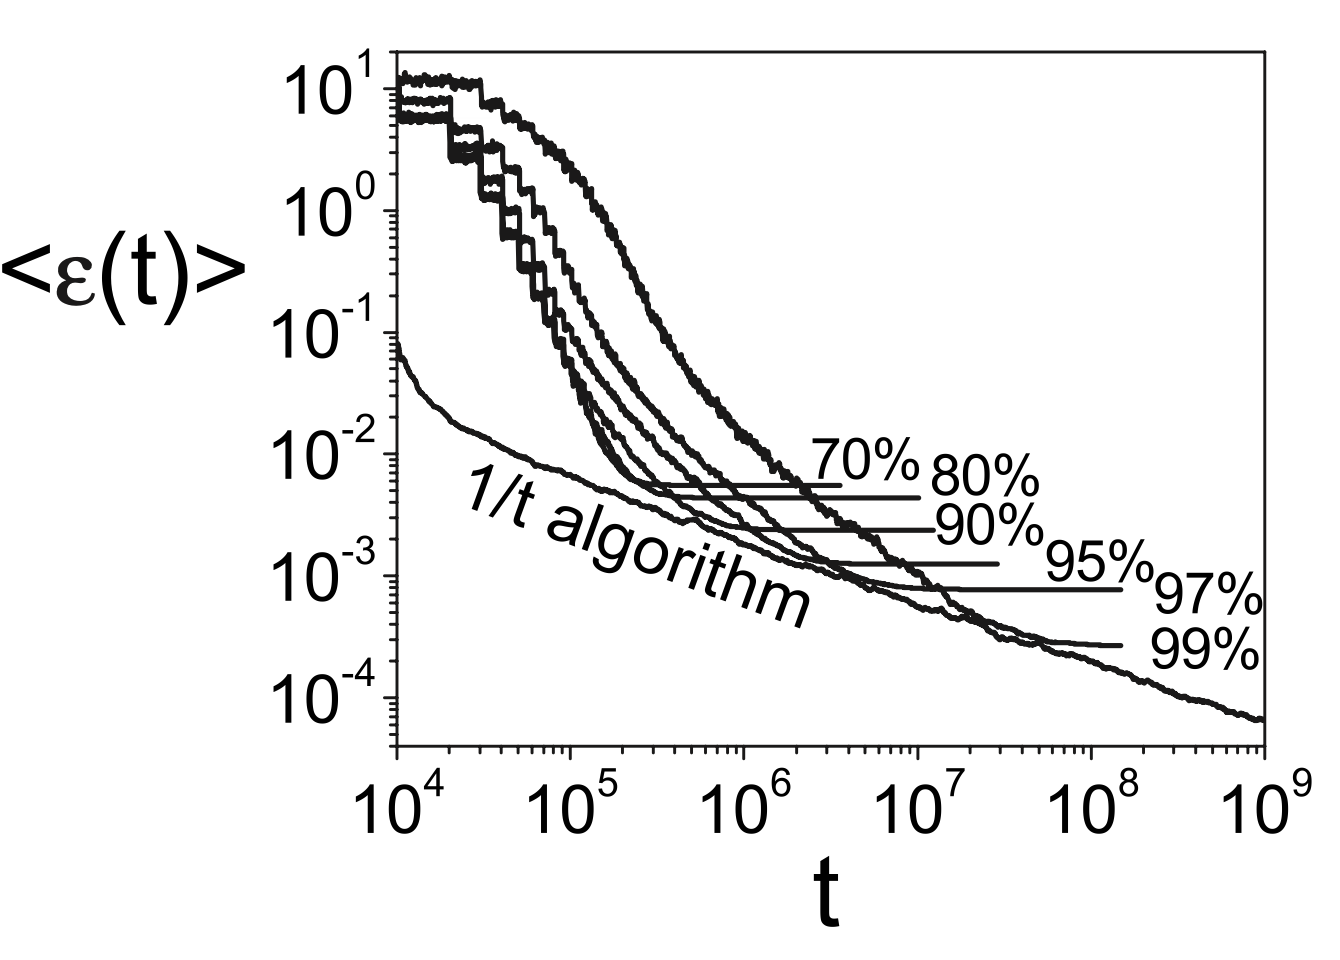
\includegraphics[scale=0.6, height=6cm]{t_paper_fig.png}
	\caption{Comparison between the mean error computed by the original WL for different flatness criteria and the mean error calculated using the $1/t$ time-dependent algorithm for a L8 SS Ising lattice. Taken from .}
	\label{t_algorithm}
\end{figure}

Despite this, the WL method has become the go-to method for DoS and JDoS estimation, because of its efficiency and ability to sample the whole phase space even if the estimation of the JDoS is not the most precise. It has been applied to magnetic systems like the Ising model, Lennard-Jones fluid simulations, biologic processes, etc.













	\chapter{Flat Scan Sampling}

	Background for the Flat Scan Sampling (FSS) method and a general description are presented along with the writers C++ implementations and an analysis of the single core and parallel performance.

\section{Background}

	The author of FSS, João Amaral, had previously, in 2014, proposed a new method to estimate the JDoS, Random Path Sampling (RPS).  The RPS was implemented in high performance languages and extensively studied by Nuno Fortunato.  (citar)
	
\begin{figure}[h]
	\centering
	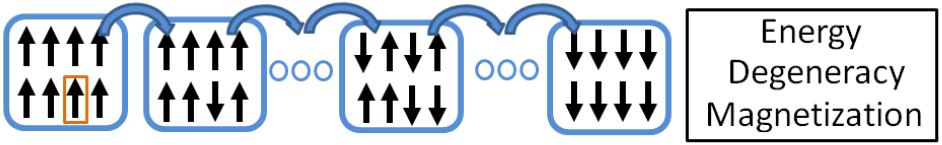
\includegraphics[scale=0.35]{rps_diagram.png}
	\caption{Scheme of how the Random Path Sampling method works.}
	\label{rps_dia}
\end{figure}
	
	The RPS method departs from the premise that by starting on an extreme magnetization point in the phase space, generally all spins up $(M)$, and successively flipping one spin down at each step of the random walk, we arrive at the other end of the phase space $(-M)$. Process illustrated in Figure \ref{rps_dia}. Performing $R$ sweeps of the phase space generate a histogram that is flat in magnetization and we can obtain the JDoS by 
\begin{align}
	H(E, M)/R &= P(E, M), \\
	\Omega(M) \times P(E, M) &= g(E, M).
\end{align}
$\Omega(M)$ is defined in Equation \ref{norm_fact}.

	The idea for FSS departs from the basic mechanism of RPS, in the sense that it is a method that estimates the JDoS by a sequential sweep of the phase space magnetization by magnetization. However the way of that both methods sample the phase space is completely different. The FSS takes a similar approach to the WL method, in the sense that a random walk with probability proportional to the inverse of the DoS is performed, a flat energy random walk.
	
	\pagebreak

\section{Algorithm}

	The Flat Scan Sampling method stems from the observation that if  the DoS at a certain magnetization $M_q$ is known, by performing a random walk the energy space $(E, M_q)$, with a probability proportional to the inverse of the DoS $\frac{1}{g(E)}$, called a flat energy random walk, and by sampling a set number of statistically diverse configurations for each energy value the DoS at the next magnetization $M_{q+1}$ can be estimated. 
This is possible because at each step of the random walk we perform a scan, i.e., in a sequential manner, we flip and unflip each spin in our configuration obtaining information about the DoS at the next magnetization, $g(E, M_{q+1})$. 
The value of $g(E_j, M_{q+1})$ is then computed through the value of $g(E_i, M_q)$ by the following equation
\begin{equation}\label{eq:FSS_JDoS}
	g(E_j, M_{q+1}) = g(E_i, M_q) \times \text{fraction of configurations}.
\end{equation}

\begin{figure}[h]
	\centering
	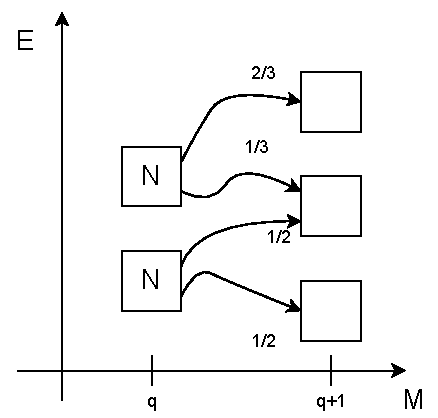
\includegraphics[scale=0.55]{fss_diagram.pdf}
	\caption{Scheme of how the Flat Scan Sampling works.}
	\label{fss_dia}
\end{figure}

Shown in Figure \ref{fss_dia}, the fraction of configurations corresponds to the fraction of the scanned configurations in the random walk that contributed to the estimation of the DoS at the next magnetization. This way, the JDoS is computed sequentially by starting at a known DoS in the phase space, such as all of the spins up $(M)$, and sweeping the whole phase space magnetization by magnetization until we arrive at the configuration where all of the spins are down $(-M)$.

The principal parameter of the method is the maximum number of samples for each point in the energy space, known as REP. In later section new parameters will be introduced to try to make the estimation more accurate while sacrificing some performance.  There will be also an extensive study of how this parameters affects the precision of the JDoS and wall time.

The algorithm can be written in the following steps:
\begin{enumerate}
\item Choose a magnetization value where $g(E, M_q)$ is known, usually magnetization where the spins all up/down;
\item Generate a certain configuration in that magnetization and compute its energy, $E_i$;                                                                                                                                       
\item Choose a spin to flip down and another one to flip up and compute the energy of the new configuration, $E_j$;
\item Accept the new configuration with a probability $\min(1, g(E_i)/g(E_j))$;
\item Sequentially flip each spin in the configuration, taking the system from the state $(E_i, M_q)$ to $(E_j, M_{q+1})$ and accumulate a histogram $H(E_i, E_j)$ and unflip the spins;
\item If the all of the number of sampled states per $(E,M_{q})$ pair is equal to REP, stop the simulation and compute the DoS at $q+1$ by using Equation \ref{eq:FSS_JDoS}. Where the fraction of configurations is now equal to $H(E_i, E_j)/\sum_j(H(E_i,E_j))$.
\end{enumerate}

\section{CPU Implementation}

	For single core and message passing interface (MPI) implementations, C++ was the preferred because of its speed and optimization over python or MatLab, and modularity, over C. The random number generator (RNG) used was the xoshrio256**.

	Before the description of the implementation let us define the function that handles the scan. This should be performed each step of the simulation. The scan is defined as flipping each spin in the configuration, measuring the new energy and registering the change in state $E_i \rightarrow E_j$ in the histogram. Thus, this operation can be implemented with a for cycle running from $0$ to $N$, the number of spins.
\begin{algorithm}
	\begin{algorithmic}[1]
	\Function{\texttt{scan}}{\texttt{configuration}}	
		\For {\texttt{idx = 0,1,..., N-1}}
			\State flip the spin \texttt{idx} spin down
			\State compute the new energy \texttt{Ej}
			\State \texttt{H(Ei, Ej)++}
			\State flip the spin \texttt{idx} spin up
		\EndFor
	\EndFunction
	\end{algorithmic} 
\end{algorithm} 

	The actual implementation follows the base-line algorithm described in the last section. By knowing that the JDoS is symmetric, to save computing time, we can estimate only half of the JDoS and after the simulation mirror it. Here \texttt{qmax} is the index of the last magnetization in our computation. The variable \texttt{hist(E)} is used to count how many configurations were sampled in each point of the energy space. We only stop when every point has sampled REP microstates. In pseudo-code it can be written as follows 
	
\begin{algorithm}
	\begin{algorithmic}[1]
		\For {\texttt{q=0,1,...,qmax}}
		 	\State set \texttt{hist(E) = 0} and \texttt{H(Ei,Ej)=0}
		 	\State generate random configuration with \texttt{M=Mq} and compute its energy \texttt{Ei}
		 	\State \texttt{scan(configuration)}
		 	\State \texttt{hist(Ei)++}
		 	\While {\texttt{min(hist(E) < REP)}}
		 		\State flip one random spin down
		 		\State flip one random spin up
		 		\State compute the energy of the new configuration \texttt{Ej}
		 		\State set \texttt{ratio = min(g(Ei)/g(Ej))}
		 		\If {\texttt{rand() < ratio}}
					\State accept new configuration
				\Else
					\State reject new configuration
		 		\EndIf
		 		\If {\texttt{hist(Ei) < REP}}
		 			\State \texttt{hist(Ei)++}
			 		\State \texttt{scan(configuration)}
		 		\EndIf
		 	\EndWhile
		 	\State set \texttt{g(E,Mq+1) = g(E,Mq) * H(Ei, Ej) / sum(H(:,Ej))} 
		 \EndFor
	\end{algorithmic} 
\end{algorithm}

	This implementation has the same problem as the original WL method. We sample successive configurations, thus reducing statistical accuracy and increasing correlation between scans. This way, a new parameter that reduces correlation between scanned configurations is proposed. It is called skip and acts the same way as the parameter $S$ in the WL. We only sample configurations that are distanced by skip steps in the random walk. Only line 17 is modified by the addition of "and \texttt{k \% skip = 0}". Usually this value is set equal to the number of spins in the system, $N$.
	
\section{Validation and Convergence}

\begin{figure}[h]
	\centering
	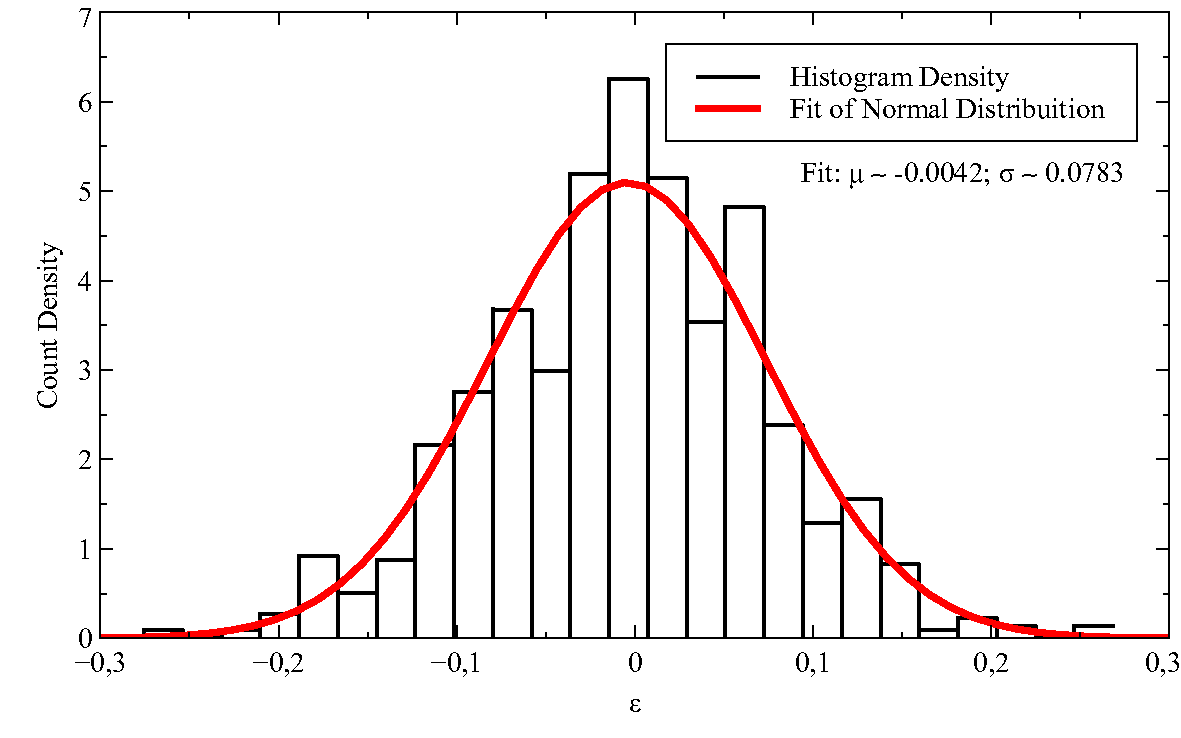
\includegraphics[scale=0.5]{convergence_validation/validation_convergence_01.pdf}
	\caption{Scheme of how the Flat Scan Sampling works.}
\end{figure}

\begin{figure}[h]
	\centering
	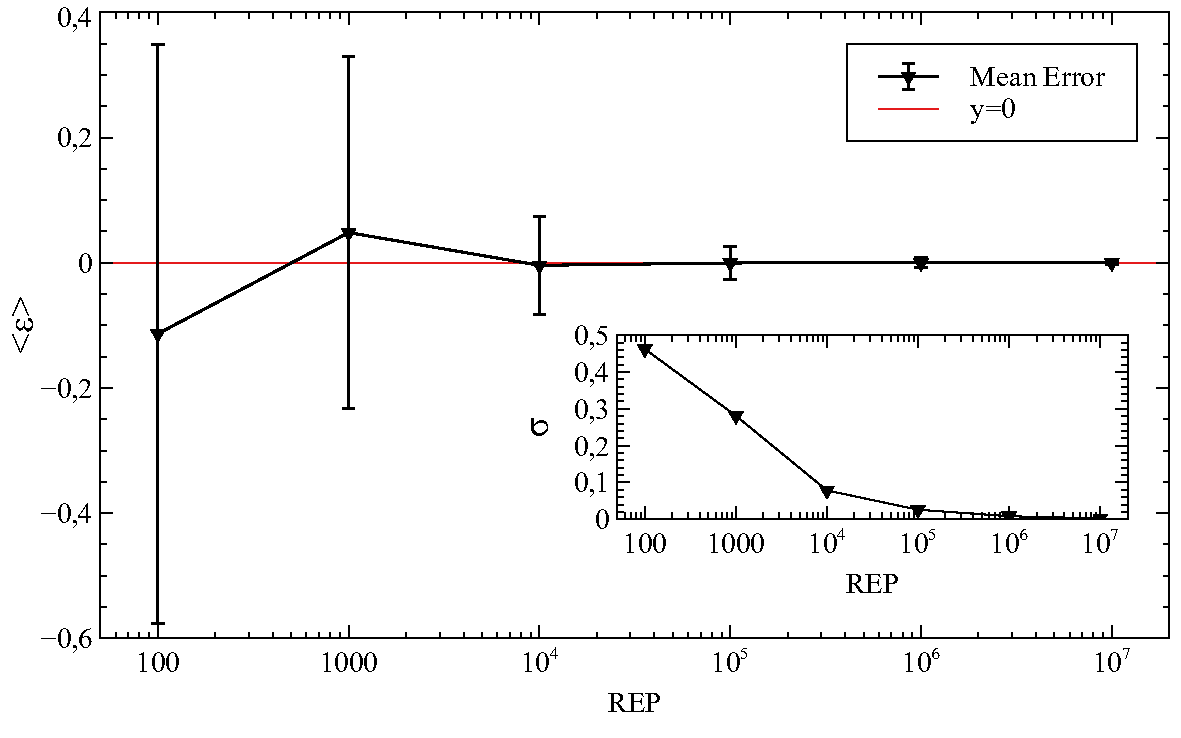
\includegraphics[scale=0.5]{convergence_validation/validation_convergence_02.pdf}
	\caption{Scheme of how the Flat Scan Sampling works.}
\end{figure}

\begin{figure}[h]
	\centering
	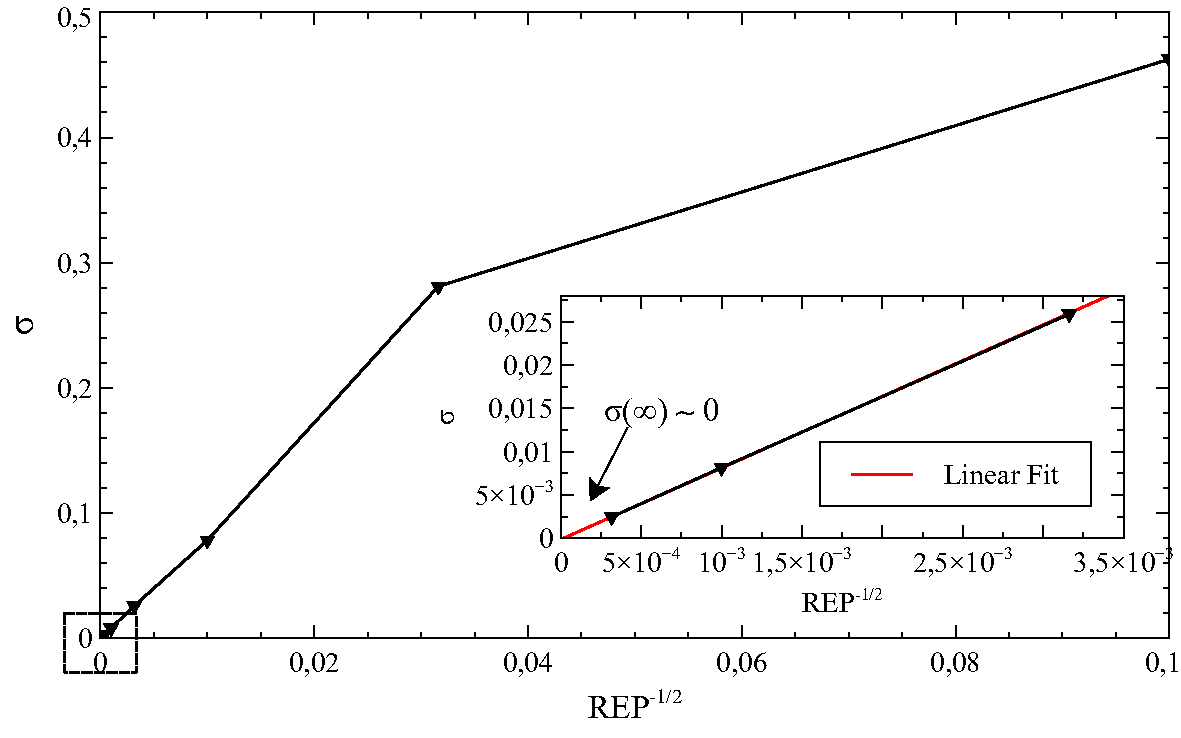
\includegraphics[scale=0.5]{convergence_validation/validation_convergence_03.pdf}
	\caption{Scheme of how the Flat Scan Sampling works.}
\end{figure}

\begin{figure}[h]
	\centering
	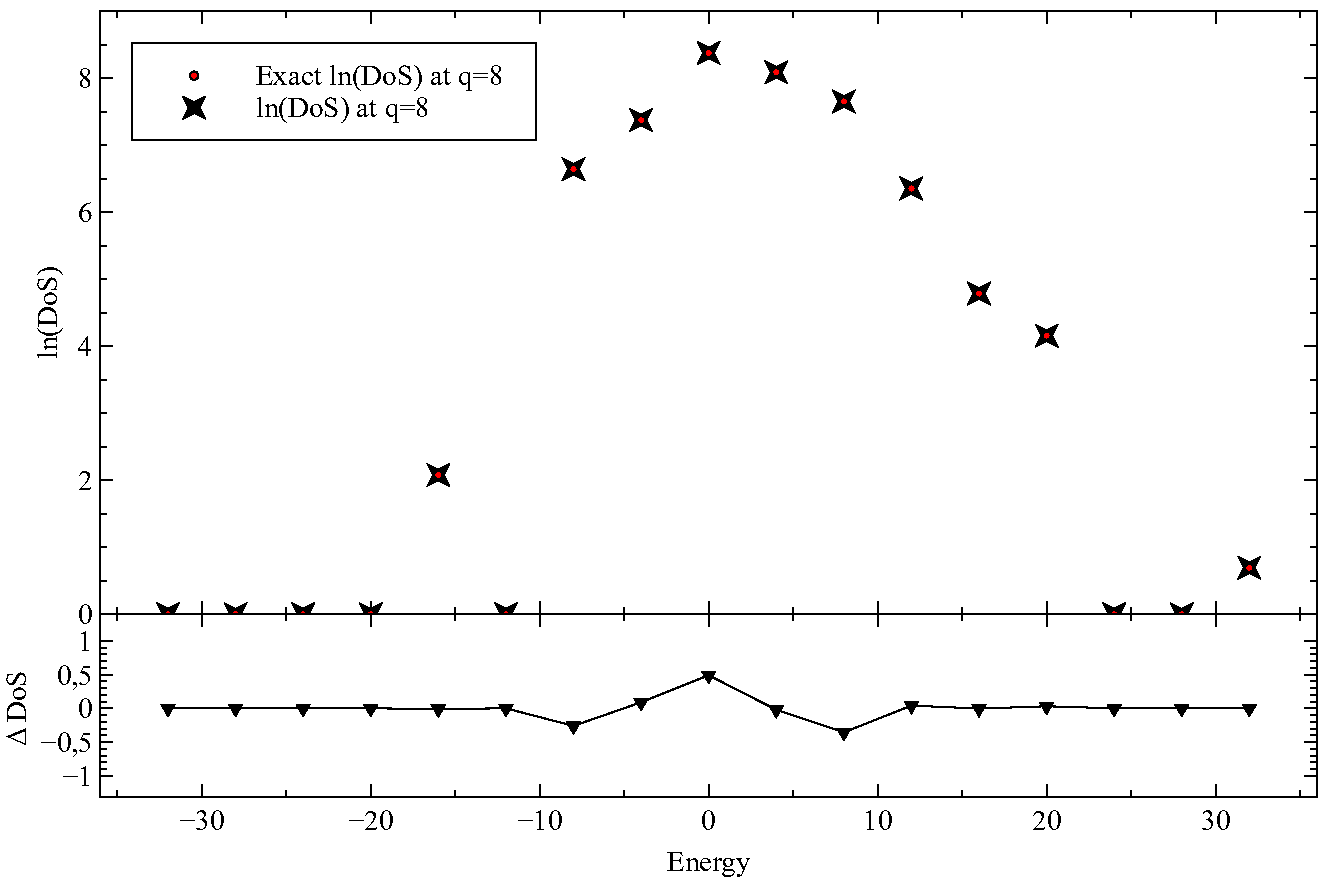
\includegraphics[scale=0.5]{convergence_validation/validation_convergence_04.pdf}
	\caption{Scheme of how the Flat Scan Sampling works.}
\end{figure}

\begin{figure}[h]
	\centering
	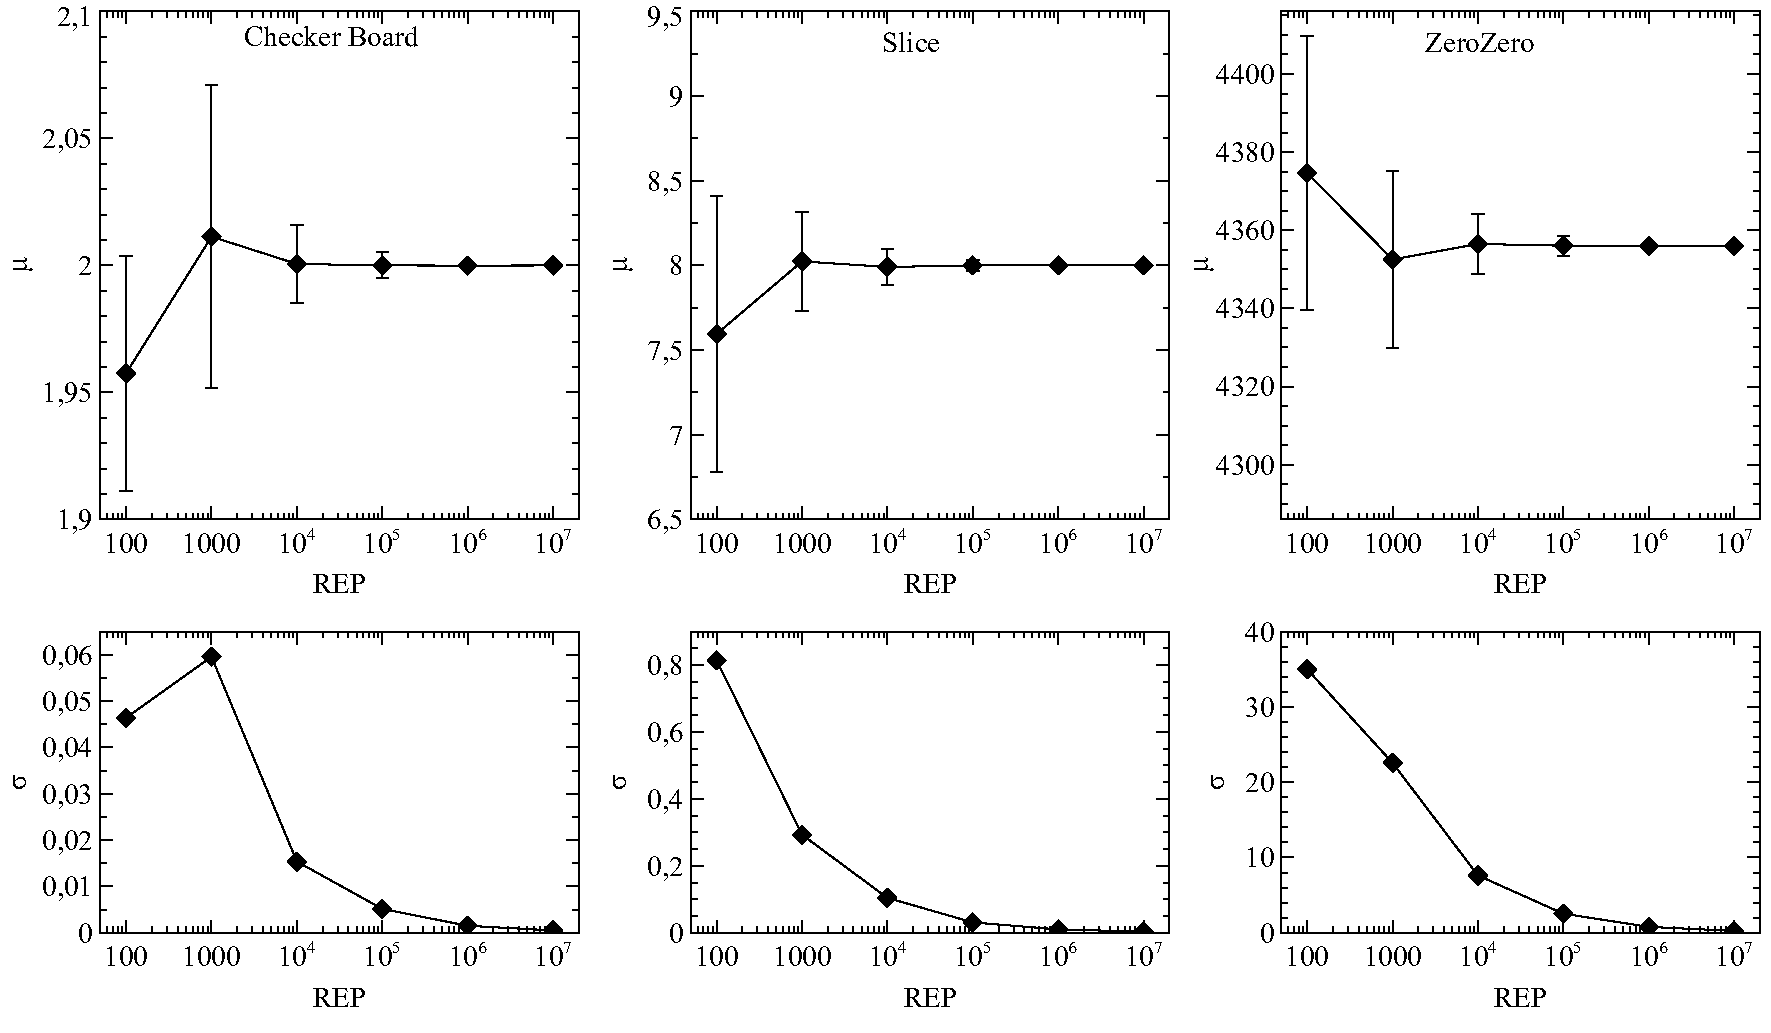
\includegraphics[scale=0.5]{convergence_validation/validation_convergence_05.pdf}
	\caption{Scheme of how the Flat Scan Sampling works.}
\end{figure}

\section{Comparison with Wang-Landau}

























	\chapter{Thermodynamics and Finite Size Scaling}
	\chapter{Thermodynamics and Finite Size Scaling}

	In this Chapter,  a comparison between mean and exact thermodynamic variables is presented along with the estimation of the Curie temperature for the infinite lattice.

	Firstly one important note on thermodynamic calculations. Extracting thermodynamic information from the JDoS can be a difficult process, specially when trying to study large systems. Although the formulas from Chapter 1 are easy to understand, the problem arrives when trying to actually compute the partition function and consequent Boltzmann factors for the ensemble average variables. 
	
	For large systems, the values from the JDoS are very large, for instance, for an L16 SS Ising system, some of the values of the JDoS are of the order $10^{74}$. We can not keep summing and multiplying these values to compute $Z$, since we run into overflow errors. For low temperatures we run into the same error, since the exponential gets very large. Instead we have to work with the logarithms of these functions to extract the thermodynamics out of the JDoS. We can use the following observation,
\begin{equation}
	\ln \left[  \sum_i a_i \right] = \ln(a_0) + \ln\left[ 1 + \sum_{i \neq 0} \frac{a_i}{a_0} \right]
\end{equation}

\section{Mean and Exact Thermodynamic Variables}

	As previously mentioned in Chapter 1, we can calculate thermodynamic variables from the JDoS in two different ways. One by using the ensemble averages through the partition function and Boltzmann factor and another by using the minimum of the Helmholtz free energy. For three different square lattice system sizes, these thermodynamic quantities can be seen in Figure \ref{thermo_4}. For the $C_{minF}$, there is only one size since smaller sizes give very inaccurate results due to numerical differentiation, Equation \ref{C_min}.
	
	We would expect that the thermodynamic quantities computed by these two equivalent ways would yield similar results. By a quick analysis of Figure \ref{mod_M} and \ref{M} we can see that the magnetization curves computed by the two methods are not that similar. The $\langle |M| \rangle$ has a flatter curve while the $M_{minF}$ has a more pronounced curve, where you can better see the phase transition. If we kept increasing the number of spin particles in our simulations, eventually these two ways would give us very similar results, and, for the infinite lattice, they would be equivalent and equal to the Onsager solution. 
\begin{figure}[h]
	\centering
	\subfigure[]{
		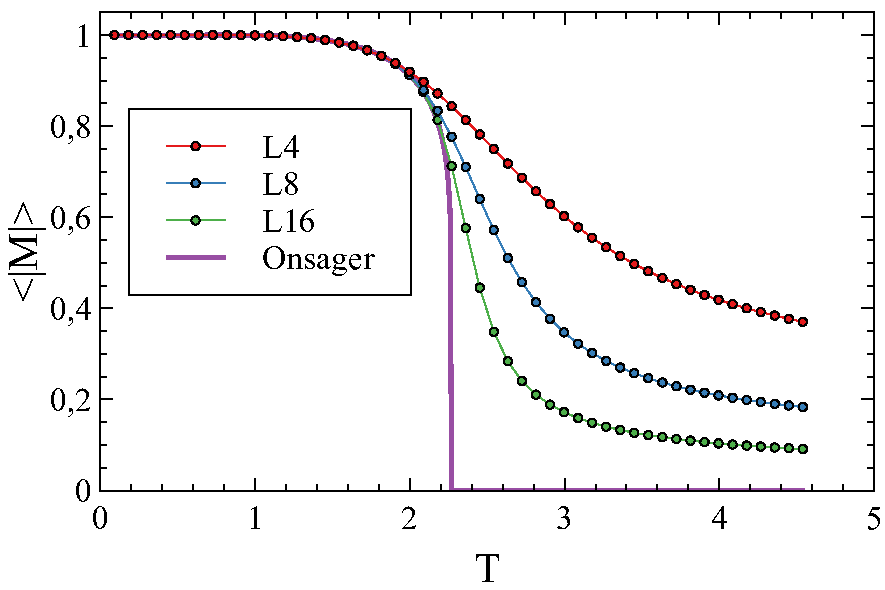
\includegraphics[scale=0.48]{thermodynamics/thermodynamics_finite_size_03.pdf}
		\label{mod_M}
	}	
	\subfigure[]{
		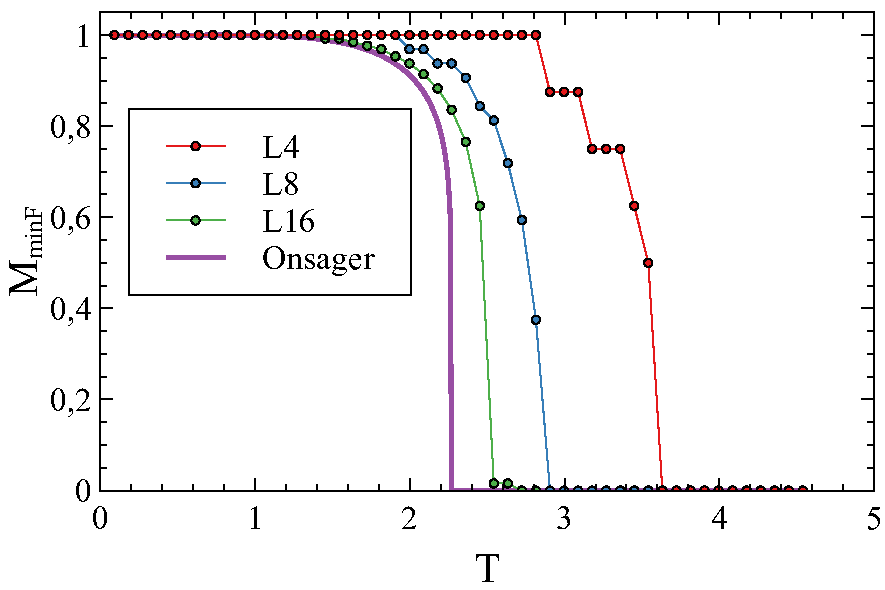
\includegraphics[scale=0.48]{thermodynamics/thermodynamics_finite_size_02.pdf}
		\label{M}
	}	
	
	\subfigure[]{
		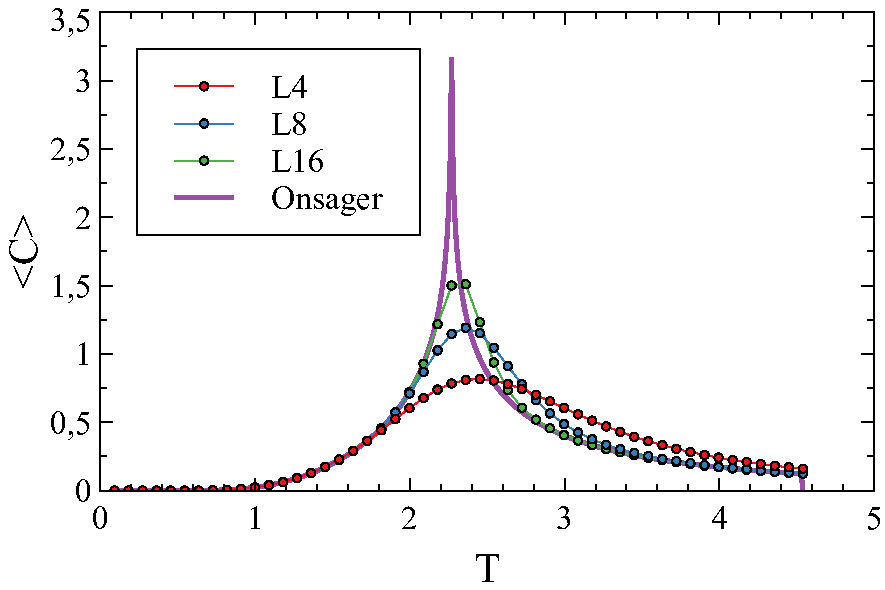
\includegraphics[scale=0.48]{thermodynamics/thermodynamics_finite_size_05.pdf}
		\label{mean_C}
	}	
	\subfigure[]{
		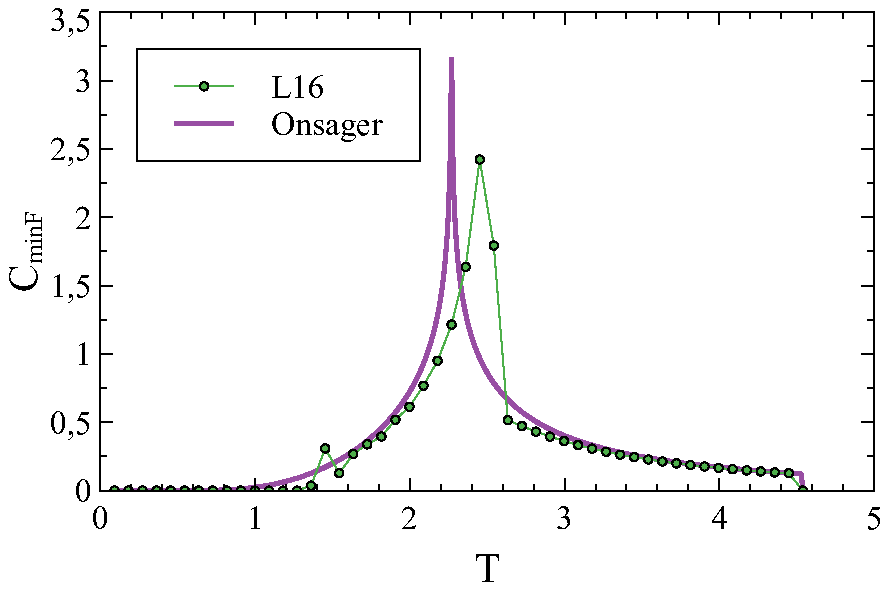
\includegraphics[scale=0.48]{thermodynamics/thermodynamics_finite_size_04.pdf}
		\label{C}
	}
	\caption{Thermodynamics for 3 different lattice sizes compared with the exact solution by Onsager. (a) $\langle |M| \rangle$. (b) $M_{minF}$. (c) $\langle C \rangle$. (d) $C_{minF}$.}
	\label{thermo_4}
\end{figure}
	Another noteworthy aspect is the Curie temperature $T_C$ that we can extract from these two curves. The point in which a phase transition occurs is the inflexion point, therefore the point where the first derivative has a relative extrema. In Table \ref{TC_table} there can be seen the Curie temperatures estimated through the two magnetization curves for the different system sizes. 

\begin{table}[h]
\centering
\caption{Curie temperature estimated by the $\langle |M| \rangle$ and $M_{minF}$ for the three different lattice sizes and their respective error. The first derivative of the magnetization has a curve with a similar shape of a Gaussian function. Thus the error can be estimated considering the half height width.}
\begin{tabular}{c|ccc|ccc}
L  & $T_C\ \langle |M| \rangle$ & $\Delta -$ & $\Delta +$ & $T_C\ M_{minF}$ & $\Delta -$ & $\Delta +$ \\ \hline
4  & 2.542                                                 & 0.726                  & 0.908         & 3.541           & 0.091                  & 0.091                \\
8  & 2.452                                                 & 0.454                   & 0.363                  & 2.815           & 0.182         & 0.091                  \\
16 & 2.361                                                 & 0.272                  & 0.182                  & 2.452           & 0.091                  & 0.091                 
\end{tabular}
\label{TC_table}
\end{table}

	The Curie temperatures taken from the average and exact thermodynamic variables are much different. The $T_C \langle |M| \rangle$ is closer to the $T_C$ for the infinite lattice but $T_C\ M_{minF}$ has much less statistical error thus it is a more precise value, since the magnetization curve is more pronounced.
	
	The mean specific heat and the specific heat obtained from the minimum of $F$, Figure \ref{mean_C} and \ref{C},respectively, have similar properties as the magnetization. The mean heat capacity has a smoother curve compared to the Onsager solution while the exact specific heat has a curve similar to the Onsager solution where the phase transition and Curie temperature are more pronounced.

\pagebreak

\section{Estimating $T_C$ for the Infinite Lattice}

	The estimation the Curie temperate for the infinite system can be obtained by two different methods \cite{Landau_Book}. The first method relies on knowing the Curie temperature for each $L$ for example the peak on the heap capacity of by the differentiation of the magnetization. This $T_C(L)$ defines a phase transition in the finite lattice. Thus we can use the linear relation
\begin{equation}\label{TC_reg_exp}
	T_C(L) = T_C(\infty) + cL^{-1/\nu},
\end{equation}
where $\nu$ is equal to unity to consider the Onsager solution, $T_C\approx2.269$ \cite{Onsager1944}.
Another way is to use the fourth order cumulant $U_L$, known as the Binder cumulant, defined as
\begin{equation}
	U_L(T) = 1 - \frac{\langle M^4 \rangle}{3\langle M^2 \rangle^2}.
\end{equation}
For a infinite system size, $L\rightarrow\infty$, the cumulant takes a value of 0 for $T>T_C$ and $2/3$ for $T<T_C$.
Plotting the Binder cumulant for different system sizes, the curves all cross a point. The temperature of this point is an estimation of the Curie temperature for the infinite lattice. The accuracy of these two methods greatly improves if larger system sizes are considered.

\begin{figure}[h]
	\centering
	\subfigure[]{
		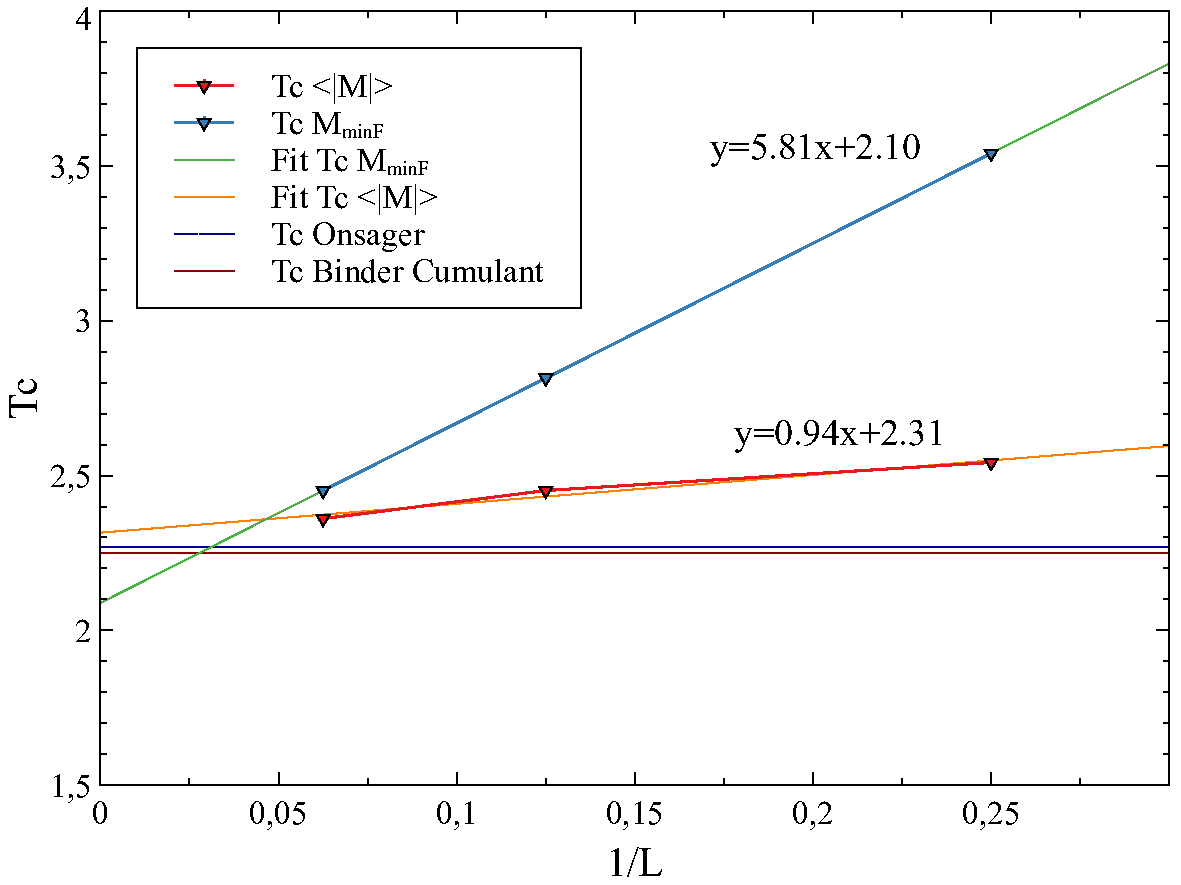
\includegraphics[scale=0.37]{thermodynamics/thermodynamics_finite_size_01.pdf}
		\label{TC_reg}
	}	
	\subfigure[]{
		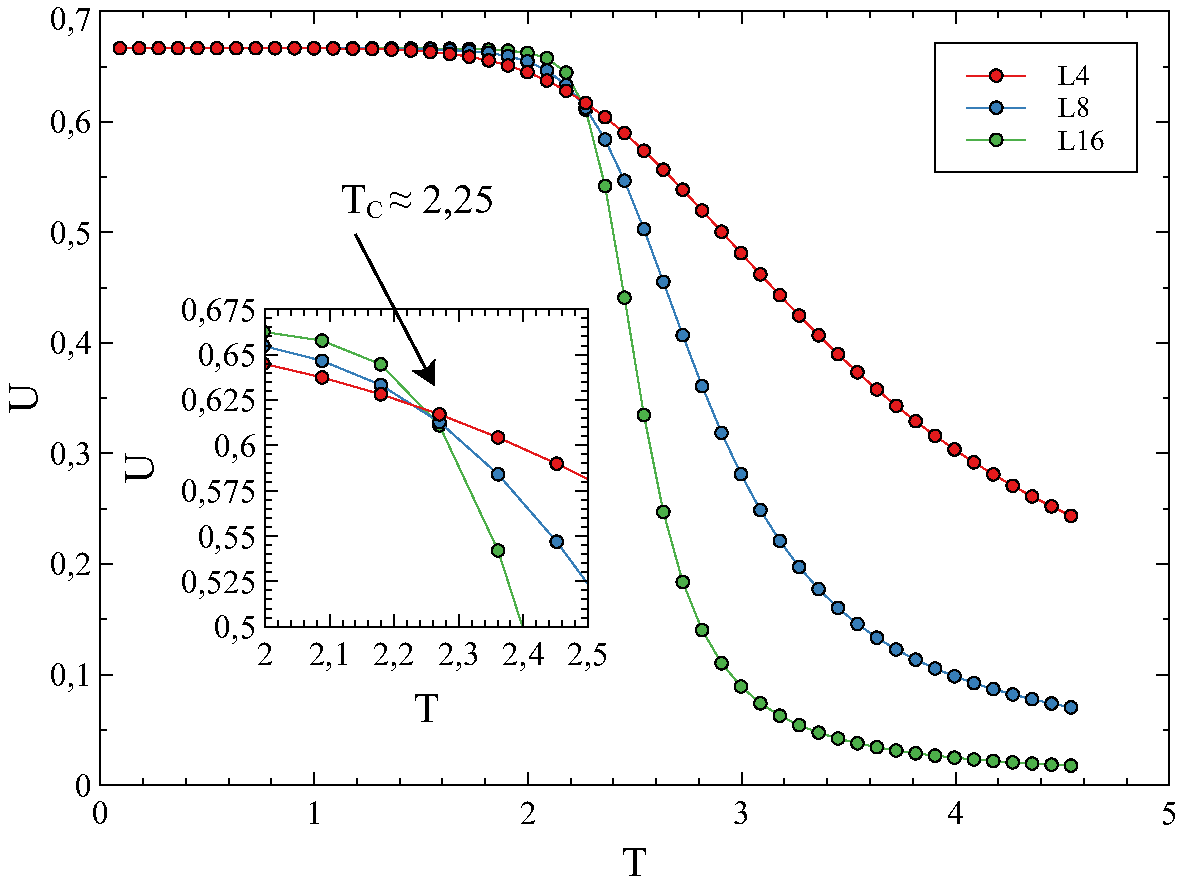
\includegraphics[scale=0.37]{thermodynamics/thermodynamics_finite_size_08.pdf}
		\label{binder}
	}
	\caption{(a) Linear regression of the $T_C(L)$ from $\langle |M| \rangle$ and $M_{minF}$ as function of $1/L$. (b) Binder cumulant for different system sizes.}
	\label{TC_inf}
\end{figure}

	For the first method, a linear regression with the $T_C(L)$ values from Table \ref{TC_table} for the two magnetization curves is presented in Figure \ref{TC_reg}. As we are only interested in the $T_C(\infty)$ from Equation \ref{TC_reg_exp}, for the the $\langle |M| \rangle$ curve, the estimated critical temperature for the infinite lattice is approximately $2.31$ while for the $M_{minF}$ is approximately $2.10$. 
	For the second method, the Binder cumulant for different L values is displayed in Figure \ref{binder}. The critical point is the point in which the curves intersect each other. This yields an estimation $T_C \approx 2.25$.
	
	For the available system sizes, the Binder cumulant gave the best results with $T_C \approx 2.25$. This is a great method of estimating the $T_C$ for the infinite lattice when we do not have results from bigger lattices, L32 or L64. The critical temperatures estimated from linear fitting the $T_C$ values form magnetizations is a good method to estimate the $T_C$ for the infinite if we have a JDoS for a bigger system.All of these estimation could be improved by considering larger systems, for example the L32 simple square.









	\chapter{Conclusion}

	A new method to estimate the Joint Density of States for the Ising was presented. It's validation, convergence and single core performance were shown and studied in great detail, finding that the method produces very precise and exact results in a small time frame. Efforts to make the simulations more presented in the form of the parameter skip. 
	
	A single core and parallel implementation based on communicating processes using MPI were developed in an high performance language. The parallel performance and scalability was studied in detail arriving to the conclusion that about 98\% of code is perfectly parallelized.
	
	A final application of the method was shown along with the comparison of mean and exact thermodynamic variables and three different methods for the estimation of the Curie temperature for the infinite lattice.
	
	This method can be generalized for the SpinS Ising model, where instead of considering spin-1/2 particles, we can consider spin-S particles. In theory this should provide better results for real materials as the total angular momentum of the composing atoms might not be 1/2.
	
\section{Future Work}	
	
	
	
	\newpage
	\pagenumbering{alph}	
	\bibliography{citations}
	\bibliographystyle{ieeetr}
	
\end{document}


